%%%%%%%%%%%%%%%%%%%%%%%%%%%%% Define Article %%%%%%%%%%%%%%%%%%%%%%%%%%%%%%%%%%
\documentclass[10pt,a4paper,openany]{article}

%%%%%%%%%%%%%%%%%%%%%%%%%%%%%%%%%%%%%%%%%%%%%%%%%%%%%%%%%%%%%%%%%%%%%%%%%%%%%%%
\usepackage[utf8]{inputenc}
\usepackage[T1]{fontenc}
%%%%%%%%%%%%%%%%%%%%%%%%%%%%% Using Packages %%%%%%%%%%%%%%%%%%%%%%%%%%%%%%%%%%
\usepackage{graphicx}
\usepackage{amssymb}
\usepackage{amsmath}
\usepackage{amsthm}
\usepackage{empheq}
\usepackage{mdframed}
\usepackage{booktabs}
\usepackage{lipsum}
\usepackage{ifthen}
\usepackage{graphicx}
\usepackage{color}
\usepackage{psfrag}
\usepackage{pgfplots}
\usepackage{bm}
%%%%%%%%%%%%%%%%%%%%%%%%%%%%%%%%%%%%%%%%%%%%%%%%%%%%%%%%%%%%%%%%%%%%%%%%%%%%%%%
\usepackage[colorlinks=true]{hyperref}
\hypersetup{
    colorlinks=true,
    linkcolor=blue!50!black,
    filecolor=blue!50!black,
    citecolor = green!50!black,      
    urlcolor=cyan,
}
\usepackage{mathtools}
\usepackage{amsthm}
\usepackage{empheq}
\usepackage{bm}
\usepackage{tikz}
\usepackage{subcaption}
\usepackage{multicol}
\usepackage[left=1.5cm,right=1.5cm,top=2cm,bottom=2cm]{geometry}
% Other Settings
\usepackage{wasysym}
\usepackage{ifthen}

%%%%%%%%%%%%%%%%%%%%%%%%%% Page Setting %%%%%%%%%%%%%%%%%%%%%%%%%%%%%%%%%%%%%%%

\usepackage{natbib}
\bibliographystyle{apalike}

\usepackage{enumitem}
\setlist{nolistsep}
%%%%%%%%%%%%%%%%%%%%%%%%%% Define some useful colors %%%%%%%%%%%%%%%%%%%%%%%%%%
\definecolor{ocre}{RGB}{243,102,25}
\definecolor{mygray}{RGB}{243,243,244}
\definecolor{deepGreen}{RGB}{26,111,0}
\definecolor{shallowGreen}{RGB}{235,255,255}
\definecolor{deepBlue}{RGB}{61,124,222}
\definecolor{shallowBlue}{RGB}{235,249,255}
\definecolor{vertcanard}{RGB}{0,69,78}
\definecolor{darkred}{RGB}{84,10,0}
\definecolor{saumon}{RGB}{100,49,42}
%%%%%%%%%%%%%%%%%%%%%%%%%%%%%%%%%%%%%%%%%%%%%%%%%%%%%%%%%%%%%%%%%%%%%%%%%%%%%%%

%%%%%%%%%%%%%%%%%%%%%%%%%% Define an orangebox command %%%%%%%%%%%%%%%%%%%%%%%%
\newcommand\orangebox[1]{\fcolorbox{ocre}{mygray}{\hspace{1em}#1\hspace{1em}}}
%%%%%%%%%%%%%%%%%%%%%%%%%%%%%%%%%%%%%%%%%%%%%%%%%%%%%%%%%%%%%%%%%%%%%%%%%%%%%%%

%%%%%%%%%%%%%%%%%%%%%%%%%%%% English Environments %%%%%%%%%%%%%%%%%%%%%%%%%%%%%
\newtheoremstyle{mytheoremstyle}{3pt}{3pt}{\normalfont}{0cm}{\rmfamily\bfseries}{}{1em}{{\color{black}\thmname{#1}~\thmnumber{#2}}\thmnote{\,--\,#3}}
\newtheoremstyle{myproblemstyle}{3pt}{3pt}{\normalfont}{0cm}{\rmfamily\bfseries}{}{1em}{{\color{black}\thmname{#1}~\thmnumber{#2}}\thmnote{\,--\,#3}}
\theoremstyle{mytheoremstyle}
\newmdtheoremenv[linewidth=1pt,backgroundcolor=shallowGreen,linecolor=deepGreen,leftmargin=0pt,innerleftmargin=20pt,innerrightmargin=20pt,]{theorem}{Theorem}[section]
\theoremstyle{mytheoremstyle}
\newmdtheoremenv[linewidth=1pt,backgroundcolor=shallowBlue,linecolor=deepBlue,leftmargin=0pt,innerleftmargin=20pt,innerrightmargin=20pt,]{definition}{Definition}[section]
\theoremstyle{myproblemstyle}
\newmdtheoremenv[linecolor=black,leftmargin=0pt,innerleftmargin=10pt,innerrightmargin=10pt,]{problem}{Problem}[section]
%%%%%%%%%%%%%%%%%%%%%%%%%%%%%%%%%%%%%%%%%%%%%%%%%%%%%%%%%%%%%%%%%%%%%%%%%%%%%%%
\usepackage{fancyhdr}
\renewcommand{\figurename}{\color{orange!90!black}{\textsc{Figure.}}}%
\renewcommand{\tablename}{\color{orange!90!black}{\textsc{Table.}}}%
\AtBeginDocument{\renewcommand{\ref}[1]{\autoref{#1}}}
\renewcommand{\thesection}{\arabic{section}}
\renewcommand{\thepart}{\arabic{part}}
% \renewcommand{\thechapter}{\arabic{chapter}}
% \renewcommand\thefigure{\thechapter.\arabic{figure}}
\pagestyle{fancy}
\usepackage[font={small}]{caption}
% %%%%%%%\pagestyle{fancy}%%%%%%%%%%%%%%%%%%%%%%%%%%%%%%%%%%%%%%%%%%%%%%%%%%%%%%%%%%%%%%%%%%%%%%%%
\fancyhead[LE]{Fintzi Nicolas}
\fancyhead[RE]{Internship report}
% \fancyhead[LO]{\chaptername\ \thechapter. \leftmark}
\fancyhead[CO]{}
\fancyhead[RO]{}
% \fancyfoot[C]{\thechapter}
%%%%%%%%%%%%%%%%%%%%%%%%%%%%%%% Title & Author %%%%%%%%%%%%%%%%%%%%%%%%%%%%%%%%
\title{Calculation note}
\author{Fintzi Nicolas}
%%%%%%%%%%%%%%%%%%%%%%%%%%%%%%%%%%%%%%%%%%%%%%%%%%%%%%%%%%%%%%%%%%%%%%%%%%%%%%%
\newcommand{\size}{0.4}
\newcommand{\sizebis}{0.5}
\setlength{\columnsep}{20pt}
%%%%%%%%%%%%%%%%%%%%%%%%%%%%%%% My commands %%%%%%%%%%%%%%%%%%%%%%%%%%%%%%%%
\newcommand{\reff}[1]{Figure \ref{#1}}
\newcommand{\refq}[1]{Equation \ref{#1}}
\newcommand{\reft}[1]{Table \ref{#1}}
%%%%%%%%%%%%%%%%%%%%%%%%%%%%%%%%%%%%%%%%%%%%%%%%%%%%%%%%%%%%%%%%%%%%%%%%%%%%%%%
\begin{document}
\maketitle
\tableofcontents

\part{First moment for a deformable particle}
\cite{batchelor1970stress}

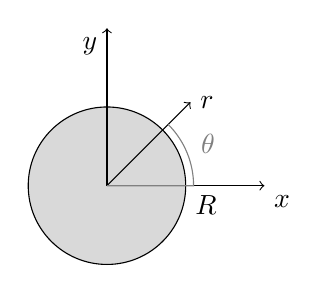
\begin{tikzpicture}
    \draw[fill=gray!30] (0,0)circle(1);
    \draw[->](0,0) --++ (2,0)node[below right ]{$x$}node[midway,below right]{$R$};
    \draw[->](0,0) --++ (0,2)node[below left ]{$y$};
    \draw[->](0,0) --++ (45:1.5)node[right]{$r$};
    \draw[gray](0,0) --++ (0:1.1)arc(0:45:1.1)node[below right]{$\;\;\;\theta$};
\end{tikzpicture}

The coordinate system can be expressed as follows :
\begin{equation}
    \left\{
    \begin{tabular}{c}
        $x =r\cos{\theta}$\\
        $y =r\sin{\theta}$
    \end{tabular}
    \right.
\end{equation}

Let's compute the volume of the circle :
\begin{equation}
    V = \int_S dS = \int_0^{2\pi}\int_0^R rdrd\theta = \pi R^2
\end{equation}
Now we can compute the position of the center of gravity with :  
\begin{align}
    \bar{x}  = \frac{1}{V}\int_S x dS = \frac{1}{V}\int_0^{2\pi}\int_0^R r^2\cos{\theta} drd\theta = 0\\
    \bar{y}  = \frac{1}{V}\int_S y dS = \frac{1}{V}\int_0^{2\pi}\int_0^R r^2\sin{\theta} drd\theta = 0
\end{align}
thus the mean position is noted $\bar{x_i} = m_1^{x_i}/m_0$.
Then let's calculate the standard deviation around the mean.
This is also called the momentum tensor. 
\begin{align}
    \bm{I}  = \left[
        \begin{tabular}{ccc}
            $\iiint (y'^2 +z'^2)dm$&$-\iiint (x'y')dm$&$-\iiint (x'z')dm$\\
            $-\iiint y'x' dm$&$\iiint (x'^2 +z'^2) dm$&$-\iiint (y'z')dm$\\
            $-\iiint z'x' dm$&$-\iiint x'y' dm$&$\iiint (y'^2 +x'^2)dm$\\
        \end{tabular}
    \right]
\end{align}
with $x_i' = x_i - \bar{x_i}$.

If we define the Gyration (or shape) tensor as :
\begin{equation}
    G_{ij} = \int \bm{x_i'}\bm{x_j'} dV.
\end{equation}
If the solid is homogeneous we can express $\bm{I}$ such that : 
\begin{equation}
    \bm{I} = \rho\left[\text{Tr}(\bm{G})\bm{\delta} - \bm{G}\right],
\end{equation}
with $\rho$ the density of the solid. 
Notice that $\bm{I}$ is in fact the deviatoric part of $\bm{G}$.  
\begin{definition}
    Let $\bm{G}$ be a gyration tensor. 
    For a given set of eigen vectors $\bm{v}_i$ and eigen values $\lambda_i$ (one for each dimension indexed by $i$). 
    $$\bm{G}\bm{v}_i = \lambda_i \bm{v}_i$$
    Physically, the eigne values represent the aspect of giration squered in each direction hold by the eigen vectors. 
    Thus, if we note $R_g^i$ the aspect of gyration $i$ we have.
    $R_g^i = \sqrt\{\lambda_i\} $
\end{definition}
Any flow around a point $O$ can be expressed at the second oder as an expension such that \citep{guazzelli2011} : 
\begin{equation}
    \bm{u}(\bm{x}) = \bm{u}(\bm{x_0}) + \bm{\nabla}\bm{u}(\bm{x})(\bm{x} - \bm{x}_O) + \mathcal{O}(\bm{x}^2)
\end{equation}
Then the gradient of the velocity tensor can be decomposed into a symetric part $\bm{E}$, and an antisymmetric part $\bm{\Omega}$.
\begin{align*}
    \bm{\Omega} = \frac{1}{2}\left[\bm{\nabla u} -\bm{\nabla u}^T\right]\\
    \bm{E} = \frac{1}{2}\left[\bm{\nabla u} +\bm{\nabla u}^T\right]
\end{align*}
$\bm{E}$ represent the rate of strain and $\bm{\Omega}$ the vorticity. 
Note that we can recover the pseudo vector representing the rotational velocity with the followng relation :
\begin{equation*}
    \bm{\omega} = -\frac{1}{2} \epsilon_{ijk}\Omega_{jk} = \frac{1}{2} \left(\bm{\nabla}\times \bm{u}\right)
\end{equation*}
In the following part we make use of the divergence theorem to calculate the integrale of the force, torque and stresslet as volume integral. 


\subsection{Calculation of the mean kinetic quantity}
The aim is to calculate from a velecity feild $\bm{u}$ the mean velocity, rotation and strain inside a given volume of fluid $V_p$.
Let's note $\bm{U_p},\omega_p$ and $\dot{\gamma}_p$, the respectively, mean velocity of the particle, the mean rotaion and the mean strain rate of the particle. 
Also let's note the corresponding quandtity $\bm{F_p}$, $\bm{L_p}$ and $\bm{M_p}$, for respectively :
the force, the torque and the first moment tensor. 

Beside in Newtonnian flows $\bm{\sigma} = p\bm{\delta} +\mu\left[\bm{\nabla u + (\nabla u)^T}\right]$, but since the hydrostatics pressure will play no rôle in the 3 previous quantity we will consider only :
$\bm{\sigma} =\mu\left[\bm{\nabla u + (\nabla u)^T}\right]$
Usulay to calculate any of the previous quantity we use the surface integral form, However in this context we prefer the volume integration over $V_p$ thus we remind the following relations :
\begin{align*}
    \bm{F_p} &= \iint_{S_p} \left( \bm{\sigma}\cdot \bm{n}\right)dS = \iiint_{V_p} \left(\bm{\nabla}\cdot \bm{\sigma}\right)dV = \mu \iiint_{V_p} \left(\bm{\nabla^2 u}\right)dV \\
    \bm{L_p} &= \iint_{S_p} \bm{x'}\times\left( \bm{\sigma}\cdot \bm{n}\right)dS = \iiint_{V_p} \bm{x'}\times \left(\bm{\nabla}\cdot \bm{\sigma}\right)dV=\mu \iiint_{V_p} \bm{x'}\times \left(\bm{\nabla^2 u}\right)dV \\
    \bm{M_p} &= \iint_{S_p} \bm{x'}\otimes\left( \bm{\sigma}\cdot \bm{n}\right)dS = \iiint_{V_p} \bm{x'}\otimes\left(\bm{\nabla}\cdot \bm{\sigma}\right)dV= \mu\iiint_{V_p} \bm{x'}\otimes\left(\bm{\nabla^2 u}\right)dV 
\end{align*}
with, $V_p$ and $S_p$ the volume and surface of the particle. 
% Let's $\bm{f} = \bm{\nabla \cdot \sigma}$.
\subsubsection*{Computation of the hydrodinamical force} 
Let $\bm{F}$ be the force acting in the particle. 
From newton second law, we have the following relation :
lala
\begin{align} 
    \bm{F_p} &= m \bm{\dot{U_p}},\\
    \bm{\dot{U_p}} &= \frac{1}{m}\int_{V_p} \bm{f}dV\\
    \bm{\dot{U_p}} &= \frac{\rho}{m}\int_{V_p} \bm{\dot{u}}dV\\
    \bm{\dot{U_p}} &= \frac{1}{\int_{V_p}dV}\int_{V_p} \bm{\dot{u}}dV\\
    \bm{U_p}       &= \frac{1}{\int_{V_p}dV}\int_{V_p} \bm{u}dV\\
\end{align}
\textcolor{blue}{le passage d'une force a une acceleration (de $f$ à $\dot{u}$) est juste dimensionelle il me manque une preuve theorique. Donc je pense que les deux ne peuvent pas être facilement lié donc les ligne du mileux sont faussent}
The quantity on the right hands side be computed numerically on \texttt{basilisk}, thus once we get $\bm{U_p}$ we can easily obtain the mean drag force exercised on the particle.  

\subsubsection*{Computation of the hydrodinamical torque} 
Let $\bm{L}$ be the pseudo vector representing the toque exercised on the sphere and $\omega$ the rotational velocity of the particle.
From newton second law, we have the following relation :
\begin{align}
    \label{eq:torque}
    \bm{I} \bm{\dot{\omega_p}} &= \bm{L_p} \\
    \bm{I} \bm{\dot{\omega_p}} &= \int_{V_p} \left(\bm{x'}\times\bm{f}\right) dV\\
    \bm{I} \bm{\dot{\omega_p}} &= \rho\int_{V_p} \left(\bm{x'}\times\bm{\dot{u}}\right) dV\\
    \bm{\omega_p} &= \bm{I}^{-1} \rho\int_{V_p} \left(\bm{x'}\times\bm{u}\right) dV\\
    \bm{\omega_p} &= \left[\text{Tr}(\bm{G})-\bm{G}\right]^{-1} \int_{V_p} \left(\bm{x'}\times\bm{u}\right) dV\\
\end{align} 
\textcolor{blue}{pareil le passage de $f$ à $\bm{\dot{u}}$ ne marche pas trop}
$\bm{\omega_p}$ can be computed only by knowing the center of mass of the particle.
Moreover, it requie to inverse the inertial matix which is always invertible since $\bm{I}$ is symmetric.   
\subsubsection*{Computation of the first moment} 
Let $\bm{L}$ be the pseudo vector representing the toque exercised on the sphere and $\dot{\gamma_p}$ the mean rate of strain of the particle.
The gradient of the velocity can be defined in each point by : $\bm{\nabla \otimes u}$.
Thus, the mean rate of strain (the symmetric part of the gradient) represent the globale rate of deformation of the particle.
We need a generalized definition similar as the one which linked the torque to the rotation but for the strain and stresslet.
The analysis of tetrad geometry in polymer science \citep{Pumir2013}\citep{willen2019resolved} make use of such an expression :
\begin{equation}
    \rho\bm{G} \cdot \bm{\nabla \dot{U_p}} = \bm{M_p} \\
    \label{eq:firstmomoent}
\end{equation}
\textcolor{blue}{le gradient de $U_p$ n'est pas forcement le gradient de $U_p$ défini avt mais un tenseur aparentiere}
With $\bm{\nabla \dot{U_p}}$ coarse-grained velocity gradient tensor, or the averaged velocity gradient tensor, the same way as $\omega_p$ is the averaged vorticity vector.
In \citet{Pumir2013} they define this quantity as a discret sum of several rigid particles (this way they can predict if a cluster of particles is in average streached or in rotation). 
Moreover, this relation is defined in a kinetic context i.e. $\bm{G} \cdot \bm{\nabla U_p} = \bm{M_p}\Delta t /\rho$, but by differentiating with respect to $t$ we get back to \ref{eq:firstmomoent}. 
In our case we assume that our particle is an infinite sum of $dV$ thus we can express the first moment as an integral over the volume of the particle. 
In \ref{eq:firstmomoent} the antisymmetric part of each side times $-\frac{1}{2}\epsilon$ gives us the previous relation \ref{eq:torque}, with $\epsilon$ the Levi-Civita tensor. 
From the relation in \citet{Pumir2013} :
\begin{align*}
    \rho\bm{G} \cdot \bm{\nabla U_p} &= \bm{M_p}\Delta t /\rho \\
    \rho\bm{G} \cdot \bm{\nabla U_p} &= \rho \int_{V_p} \left(\bm{x'}\otimes\bm{u'}\right)dV \\
    \bm{\nabla U_p} &= \bm{G}^{-1}  \int_{V_p} \left(\bm{x'}\otimes\bm{u' }\right)dV \\
\end{align*} 
Thanks to \ref{eq:firstmomoent} one can compute the volume averaged firstmomoent. 
The gradient of the velocity tensor has been calculated doing similar hypothesis as the former two quandtities. 
From the averaged first moment it is possible to recover the mean stresslet $\bm{S_p}$ (which is the symmetric part of $\bm{M_p}$) as follows :
\begin{equation}
    S_p = \frac{1}{2}\left[\bm{M_p}+\bm{M_p^T}\right]
\end{equation}
Also we can define the symmetric and antisymmetric part of $\bm{\nabla U_p}$  :
\begin{align}
    \bm{\dot{\gamma}_p} &= \frac{1}{2}\left[\bm{\nabla U_p}+\bm{\nabla U_p}^T\right]\\
    \bm{\Omega_p}& = \frac{1}{2}\left[\bm{\nabla U_p}-\bm{\nabla U_p}^T\right]
\end{align}
$\bm{\dot{\gamma}_p}$ is the volume averaged rate of strain tensor which tells us if the particle is streaching, while $G$ tells us if it is streached. 
Besides, we can recover $\bm{\omega}$ with :
\begin{equation}
    \omega^P_i = -\frac{1}{2}\epsilon_{ijk}\Omega^P_{jk}
\end{equation}


\part{Balance energy equation for drops suspension}
Let's start from the one-fluid formulation of the momentum balance equation i.e. : 
\begin{equation}
    \rho \frac{\partial \bm{u}}{\partial t}+\rho\nabla\cdot\bm{uu} = 
    -\nabla p +\bm{f} +\nabla\cdot\mu\left[\nabla\bm{u}+(\nabla\bm{u})^T\right] + \bm{f}_\sigma\delta_\sigma
    \label{eq:momentumbal}
\end{equation}
Multiplying \refq{eq:momentumbal} by $\bm{u}$ gives :
\begin{equation}
    \rho \frac{\partial u^2/2}{\partial t}+\rho\nabla\cdot\bm{uu} = 
    -\bm{u}\nabla p +\bm{f} +\nabla\cdot\mu\left[\nabla\bm{u}+(\nabla\bm{u})^T\right] + \bm{f}_\sigma\delta_\sigma
    \label{eq:momentumbal}
\end{equation}

\part{Balance of surface en kinetics energy for a population of spherical droplet}

In any suspension of drops,
two bubbles tend to merge together in order to decrease the surface energy.
Indeed, for a given volume the shape that minimize the surface energy is the spherical or circular shape in 3D or in 2D.
Thus, for a given set of drops, if we wait enough time they should all merge together and form a single bubble. 
We can define the following dimensionless parameters :

\begin{equation*}
    Ga =\frac{\rho_l\Delta\rho g d_b^3}{\mu^2_l},
\end{equation*}
\begin{equation*}
    Bo =\frac{\Delta\rho g d_b}{\sigma},
\end{equation*}
\begin{equation*}
    Re =\frac{U_b^2 d_b}{\nu_l},
\end{equation*}
\begin{equation*}
    We = \frac{BoRe^2}{Ga}=\frac{\rho_b U_b^2 d_b}{\sigma},
\end{equation*}
with $\rho_b$ the density, $U_b$ the rising velocity of the bubble and $d_b$ the diameter. 
\begin{enumerate}
    \item We can notice that when the bubbles merge they create bubbles with larger diameter while the other physical parameters stay constant. 
    \item Therefore, $We$ increase as the bubbles merge.
    \item Then at some point $We$ will reach a threshold value and the bubble will break. 
    \textcolor{blue}{Probably because there is high $\Delta E_c$ ?}
    \item When the bubble break it create a thin film or column between the two parts.
    \item The column or film exhibit Rayleigh-Taylor instability, then we see the smallest bubbles appear. 
    \item Then either the small bubbles can not merge because they are too small and the $t_d$ become too big, or they can and the loop continue.
\end{enumerate}
In order to determine the final form of the distribution function of particle size $n(L)$,
we will try to find the function $n(L)$ which minimize the total energy.
Moreover, we consider only circular or spherical drops a log-normal distribution.
Let express the kinetic energy for a given particle of size $L$. 
\begin{equation}
    E_c(L) = \frac{1}{2} \rho V_p(L) U_p^2(L) =\frac{1}{2} \rho k_v L^3 U_p^2(L) ,
    \label{eq:Ec}
\end{equation}
with $k_v$ the coefficient linking size and volume, $4/3 \pi$ for a sphere. 
Now let's express the surface tension energy,
\begin{equation}
    E_\sigma(L) = \gamma S_p(L) =\gamma k_s L^2 ,
    \label{eq:Es}
\end{equation}
with $\gamma$ the superficial surface tension. 
Then the energy balance must be : 
\begin{equation}
    E_c(L) +E_\gamma(L) = C,
\end{equation}
with C a constant. 
Let $n(L)$ be a number density of particles of size $L$ such that the number of particles include in a range $[L;L+dL]$ reads as :
\begin{equation*}
    N = n(L)dL V,
\end{equation*}
with $V$ the volume of the domain.
Therefore, the total energy reads as : 
\begin{equation}
    \int_0^\infty \left[E_c(L)  +E_\gamma(L)\right]n(L) dL = C,
\end{equation}
\textcolor{blue}{This equation is false, the energy is balance must include the dissipation}
In the physical case, we know that a threshold diameter above which the bubble break exist. 
Thus, the range of integration might be reduced.
The main constrain that we impose is the conservation of the total volume of particles $\mathcal{V}$ per unit of volume. 
We want to minimize the energy, while keeping a volume of particles constant.
Therefore, we need to minimize the functional :
\begin{equation}
    G =  \int_0^\infty E_c(L)n(L)dL + \int_0^\infty E_\gamma(L)n(L)dL - \lambda \mathcal{V},
\end{equation}
where $\lambda$ is a Lagrange multiplier.
By substituting \ref{eq:Ec} and \ref{eq:Es} it follows : 
\begin{equation}
    G =  \int_0^\infty \left(\frac{1}{2} \rho k_v L^3 U_p^2(L) n(L)\right)dL + \int_0^\infty \left(\gamma k_s L^2 n(L)\right)dL - \lambda \int_0^\infty L^3 k_v n(L) dL,
\end{equation}
\begin{equation}
    G =  \frac{1}{2} \rho k_v \int_0^\infty L^3 U_p^2(L) n(L)dL + \gamma k_s \int_0^\infty L^2 n(L)dL - \lambda k_v\int_0^\infty L^3  n(L) dL,
\end{equation}
\textcolor{blue}{check the Lagrange multiplier theory because since $\dot{n}$ doesn't appear it is a bit too much}
How to express $U_p^2(L)$ ? 
There is different scaling law However if we take \citet{tomiyama1998drag} we see that $U_p^2(L) \sim L$.

Regarding the distribution function $n(L)$ we will consider that it follows a log-normal distribution. 
Indeed, in \citet{KAMP20011363} they observe this king of distribution for bubbly flows. 
Thus, $n(L)$ reads as : 
\begin{equation}
    n(\log L) = \frac{1}{\sqrt{2\pi}\log{\sigma'}}  \exp\left[{-\frac{\log^2(L/\bar{L'})}{2\log^2{\sigma'}}}\right]
\end{equation}
With $\bar{L'}$ the mean and $\sigma'$ the width parameter. 
The $j^{th}$ moment of the distribution is defined as :
\begin{equation}
    m_j= \frac{1}{\sqrt{2\pi}\log{\sigma'}} \int_ {-\infty}^\infty L^j\exp\left[{-\frac{\log^2(L/\bar{L'})}{2\log^2{\sigma'}}}\right]d(\log L)
\end{equation}
After integration it gives :
\begin{equation}
    m_j= \bar{L'}^j\exp\left[-\frac{1}{2}j^2\log^2\sigma'\right]
\end{equation}

The first moment is kind of known since we already know the total volume (thus the mean total vol).
\bibliography{Bib/bib_bulles.bib}
\appendix
\addcontentsline{toc}{part}{Appendix}

\end{document}